\subsection{UC5 - Calcolo matrice di distanza}
    \label{uc5}
    
    \begin{figure}[htbp]
        \centering
        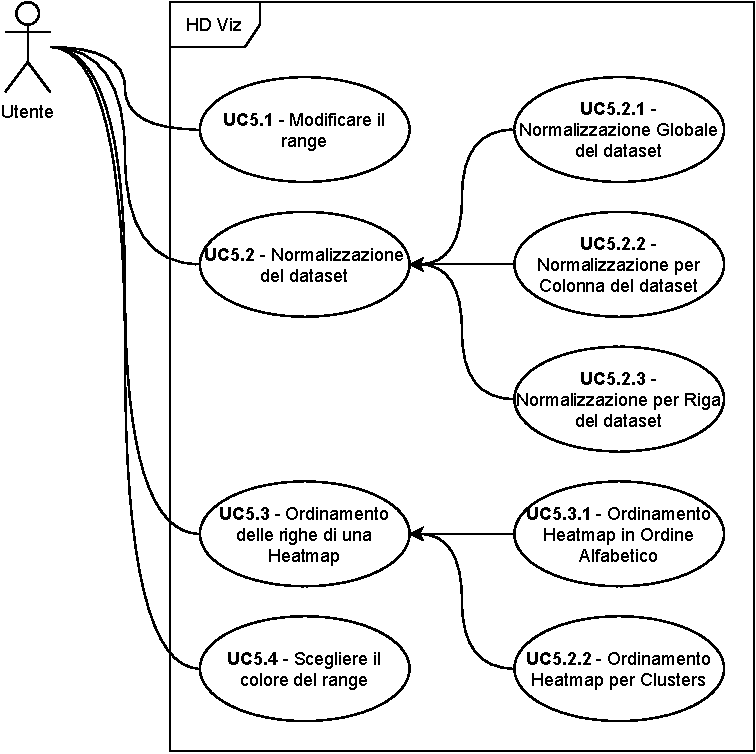
\includegraphics[width=0.45\textwidth]{source/sections/casi-uso/diagrams/uc5.pdf}
        \caption{UC5 - Calcolo matrice di distanza}
        \label{fig:uc5}
    \end{figure}
    
    \begin{itemize}
    \item \textbf{Attore}: utente;
    \item \textbf{Descrizione}: data una matrice $N \times M$ viene calcolata la distanza tra ogni riga e viene restituita all'utente una matrice di distanza N x N dove ${x_i}_j$ è la distanza tra la riga $i$ e la riga $j$ della matrice di partenza;
    \item \textbf{Precondizione}: 
    \begin{itemize}
        \item eseguito l'upload del dataset come matrice $N\times M$ (\hyperref[uc1]{UC1});
        \item selezionato Heatmap o Force Field come visualizzazione (\hyperref[uc2.2]{UC2.2} o \hyperref[uc2.4]{UC2.4}).
    \end{itemize}  
    \item \textbf{Postcondizione}: calcolata matrice di distanza $N \times N$ dove ${x_i}_j$ è la distanza tra la riga $i$ e la riga $j$ della matrice di partenza;
    \item \textbf{Scenario Principale}: 
    \begin{enumerate}
        \item l'utente seleziona il calcolo della matrice di distanza corrispondente al dataset caricato;
        \item l'utente seleziona la distanza (\hyperref[uc6]{UC6}).
    \end{enumerate}  
    \item \textbf{Inclusioni}:
        \begin{enumerate}
            \item scelta dell'algoritmo di distanza da utilizzare (\hyperref[uc6]{UC6}).
        \end{enumerate} 
    \end{itemize}